\documentclass[10pt,a4paper,twocolumn]{article}
\usepackage[utf8]{inputenc}
\usepackage[T1]{fontenc}
\usepackage[spanish,es-tabla]{babel}
\usepackage{geometry}
\geometry{margin=1.8cm,columnsep=0.7cm}
\usepackage{booktabs}
\usepackage{array}
\usepackage{url}
\usepackage{graphicx}
\usepackage{listings}
\lstset{basicstyle=\ttfamily\footnotesize, breaklines=true, columns=fullflexible}
\setlength{\parindent}{0pt}
\setlength{\parskip}{0.45em}
\setlength{\emergencystretch}{3em}
\raggedbottom
\usepackage{fvextra}

\begin{document}
\twocolumn[
\begin{minipage}{\textwidth}
\centering
{\LARGE\bfseries Caracterización y reducción de imágenes CCD\par}
\vspace{0.35em}
{\normalsize Daniel Soto Villada y Joan Mauricio Yanza Ruiz\par}
{\small [Afiliación institucional]\par}
{\normalsize [Fecha]\par}
\vspace{0.7em}
\textbf{Resumen}\par
\small
% Pendiente de completar.
\end{minipage}
\vspace{1em}
]

\section{Introducción}
La observación astronómica mediante detectores de dispositivo de carga acoplada (CCD) es una herramienta importante  para obtener información de los objetos celestes. Estos detectores convierten la luz incidente en señales electrónicas que posteriormente se almacenan en imágenes digitales. Sin embargo, las imágenes obtenidas no representan estrictamente la señal procedente del objeto observado, ya que también contienen contribuciones asociadas al  proceso de lectura, la temperatura y las variaciones de sensibilidad del detector. Por esta razón, es necesario efectuar un proceso de calibración y reducción de imagenes  que permita corregir estos efectos y obtener imágenes adecuadas para su estudio.\\

En este trabajo se realizó la reducción de imágenes CCD del cúmulo abierto Melotte 25, adquiridas con  filtros fotométricos B y V mediante una cámara CCD-FLI ML0900 en el observatorio La Silla. El procesamiento se llevó a cabo utilizando el entorno IRAF, a partir de imágenes de calibración de tipo \textit{bias}, \textit{dark} y \textit{flat}. Inicialmente, se identificaron y corrigieron las regiones de \textit{overscan} , con el propósito de delimitar el área científica de las imágenes. Posteriormente, se construyeron las imágenes maestras("master") de calibración y se aplicaron las correcciones correspondientes a las imágenes científicas.\\

Finalmente, se obtuvieron las imágenes reducidas en los filtros B y V, cuya inspección y análisis estadístico permitieron evaluar los resultados del procedimiento y reconocer las limitaciones asociadas al proceso de calibración.\\

\section{Materiales y métodos}
\subsection{Bitácora de observación}
La información de las Tablas~\ref{tab:bitacora} y~\ref{tab:noches} se extrajo
directamente de las cabeceras FITS con las tareas \texttt{imhead} y
\texttt{hselect} de IRAF:

\begin{lstlisting}
ecl> imhead Bias/domeflat_Bias_1_secs_001.fits l+
ecl> imhead MEL25_Light_B_90_secs_001.fits l+
ecl> hselect Bias/*.fits,Dark/*.fits,domeflat_B/*.fits,domeflat_V/*.fits,MEL25*.fits "$I,IMAGETYP,FILTER,EXPTIME,DATE-OBS,UT,CCD-TEMP,INSTRUME" yes > bitacora.txt
ecl> !cat bitacora.txt
\end{lstlisting}

\noindent\textbf{Parámetros fijos leídos de las cabeceras:} observatorio La
Silla; cámara CCD-FLI ML0900 (alias TUCAN, \texttt{INSTRUME='FLI CCD'});
adquisición generada por INDI; binning $1\times1$; píxel de 12\,$\mu$m; escala
de 8.252''/píxel; formato de $3056\times3056$ píxeles con dos regiones de
overscan (sobre filas y sobre columnas).

\begin{table*}[t]
\centering
\caption{Bitácora de observación resumida por tipo de imagen. Las horas están
en UT y corresponden al inicio y al cierre de cada serie.}
\label{tab:bitacora}
\footnotesize
\setlength{\tabcolsep}{3pt}
\begin{tabular}{@{}>{\raggedright\arraybackslash}p{4.3cm}lcccllc@{}}
\toprule
Archivo (patrón de nombres) & Tipo (\texttt{IMAGETYP}) & $N$ & $t_{\mathrm{exp}}$\,(s) & Filtro & Fecha y hora (UT) & $T_{\mathrm{CCD}}$\,($^\circ$C) \\
\midrule
\path{Bias/domeflat_Bias_1_secs_001-047.fits} & zero (bias) & 47 & 0  & Ha, X, V, I, U & 2024-10-25/26, 21:46:54--02:53:39 & $-24.94$ \\
\path{Dark/MEL25_Dark_90_secs_001-005.fits}   & dark        & 5  & 90 & I              & 2024-12-04, 04:28:54--04:35:41     & $-25.00$ \\
\path{domeflat_B/domeflat_Flat_B_90_secs_001-005.fits} & flat & 5 & 90 & B              & 2024-10-25, 21:53:02--21:59:53     & $-24.94$ \\
\path{domeflat_V/domeflat_Flat_V_40_secs_001-005.fits} & flat & 5 & 40 & V              & 2024-10-25, 22:01:37--22:05:08     & $-24.94$ \\
\path{MEL25_Light_B_90_secs_001.fits}         & object      & 1  & 90 & B              & 2024-12-04, 04:04:09               & $-25.00$ \\
\path{MEL25_Light_V_90_secs_001.fits}         & object      & 1  & 90 & V              & 2024-12-04, 04:04:09               & $-25.00$ \\
\bottomrule
\end{tabular}
\end{table*}

\begin{table*}[t]
\centering
\caption{Reconstrucción cronológica de las noches de observación (Paso 1).}
\label{tab:noches}
\footnotesize
\begin{tabular}{@{}lllccc@{}}
\toprule
Noche (UT) & Hora (UT) & Tipo de imagen & Filtro & $N$ & $t_{\mathrm{exp}}$\,(s) \\
\midrule
2024-10-25 & 21:46:54--21:50:54 & bias          & Ha & 20 & 0  \\
           & 21:52:34--21:52:47 & bias          & X  & 2  & 0  \\
           & 21:53:02--21:59:53 & dome flat     & B  & 5  & 90 \\
           & 22:01:37--22:05:08 & dome flat     & V  & 5  & 40 \\
           & 22:05:59--22:06:12 & bias          & V  & 2  & 0  \\
           & 23:01:52--23:02:05 & bias          & I  & 2  & 0  \\
2024-10-26 & 02:49:28--02:53:39 & bias          & U  & 21 & 0  \\
\midrule
2024-12-04 & 04:04:09           & ciencia MEL25 & B  & 1  & 90 \\
           & 04:04:09           & ciencia MEL25 & V  & 1  & 90 \\
           & 04:28:54--04:35:41 & dark          & I  & 5  & 90 \\
\bottomrule
\end{tabular}
\end{table*}

\noindent\textbf{Notas de la bitácora:}
\begin{itemize}\footnotesize
\item El archivo \path{Bias/Zero.fits} duplica el marco 001 (mismo \texttt{DATE-OBS}); se contabilizó una sola vez (47 bias únicos).
\item El filtro anotado en los bias (Ha, X, V, I, U) corresponde a la posición de la rueda de filtros al momento de leer el cero; el nivel de bias no depende del filtro.
\item Los darks se tomaron con la rueda en I; la corriente oscura es independiente del filtro.
\item Ambas imágenes de ciencia reportan el mismo \texttt{UT} en sus cabeceras (para B, \texttt{UTMIDDLE} = 2024-12-04T04:04:54.82).
\end{itemize}

\subsection{Ganancia y ruido de lectura}
La ganancia $g$ y el ruido de lectura RN se determinaron por filtro mediante el
método de la varianza de diferencias: con un par de dome flats y un par de bias
se construyen imágenes de diferencia, que eliminan toda estructura espacial
(iluminación, polvo, viñeteo) y conservan únicamente el ruido:

\begin{equation}
\sigma^2_F = \frac{\mathrm{Var}(F_1-F_2)}{2}, \qquad
\sigma^2_B = \frac{\mathrm{Var}(B_1-B_2)}{2},
\end{equation}
\begin{equation}
g = \frac{\bar{F}-\bar{B}}{\sigma^2_F-\sigma^2_B}, \qquad
\mathrm{RN} = g\,\sigma_B .
\end{equation}

\noindent Las estadísticas se calcularon sobre la región central
$[1000:2000]\times[1000:2000]$ para excluir overscan y bordes. Para el filtro B
se usaron los flats 001--002 con los bias 019--020 (contiguos en el tiempo);
para el filtro V, los flats 001--002 con los bias 023--024. El cálculo se
realizó con un script en Python (\texttt{astropy}/\texttt{numpy}).

\subsection{Ajuste y sustracción del overscan bidimensional}
Las imágenes del detector CCD-FLI ML0900 (TUCAN) presentan dos regiones de
overscan: una franja vertical en las columnas izquierdas y una franja
horizontal en las filas inferiores. Estas regiones no corresponden al área
fotosensible del detector, sino a píxeles ficticios que permiten monitorear
el nivel electrónico de lectura. Para corregir este efecto se emplearon las
tareas \texttt{colbias} y \texttt{linebias} del paquete \texttt{bias} de
IRAF, que ajustan un polinomio de Chebyshev al nivel de lectura en cada
franja y lo sustraen de la imagen científica.

\subsubsection{Identificación de las regiones de overscan}

Para determinar los límites de overscan se analizaron los perfiles medios
de columnas y filas de un dome flat B con un script en Python y
\texttt{astropy}. El archivo de prueba fue
\path{domeflat_B/domeflat_Flat_B_90_secs_001.fits}:

\begin{lstlisting}[language=Python]
import numpy as np
from astropy.io import fits

img = 'domeflat_B/domeflat_Flat_B_90_secs_001.fits'
d = fits.getdata(img).astype(float)
nc, nr = d.shape[1], d.shape[0]

col = d.mean(axis=0)    # perfil a lo largo de columnas
row = d.mean(axis=1)    # perfil a lo largo de filas
nivel_col = np.median(col[nc//3:2*nc//3])
nivel_row = np.median(row[nr//3:2*nr//3])

def limites(perfil, nivel):
    dentro = np.where(perfil > nivel*0.5)[0]
    return dentro[0]+1, dentro[-1]+1

c1, c2 = limites(col, nivel_col)
r1, r2 = limites(row, nivel_row)

print(f'Area cientifica columnas: {c1}:{c2}')
print(f'Area cientifica filas:    {r1}:{r2}')
\end{lstlisting}

\noindent La salida del script indicó:

\begin{itemize}
\item \textbf{Overscan de columnas (primera región):} franja vertical
izquierda, columnas 1:35, con nivel de lectura $\approx 1020$ ADU.
\item \textbf{Overscan de filas (segunda región):} franja horizontal
inferior, filas 1:20, con nivel de lectura $\approx 1208$ ADU.
\item \textbf{Área científica bruta:} columnas 36:3056, filas 21:3056.
\end{itemize}

\subsubsection{Corrección de la primera región (columnas) con \texttt{colbias}}

La tarea \texttt{colbias} ajusta un polinomio de Chebyshev al nivel de
lectura en la franja de overscan de columnas, lo sustrae de cada fila y
recorta la imagen al área científica definida por \texttt{trimsection}.
Los parámetros utilizados fueron:

\begin{lstlisting}
noao
imred
bias
unlearn colbias
colbias domeflat_B/domeflat_Flat_B_90_secs_001.fits TrmFlatB001.fits \
  bias="[1:35,21:3056]" trim="[36:3056,1:3056]" \
  function=chebyshev order=1 interactive=no median=no \
  low_rej=3. high_re=3.
\end{lstlisting}

\noindent\textbf{Descripción de parámetros:}
\begin{itemize}
\item \texttt{bias="[1:35,21:3056]"}: región de overscan de columnas
utilizada para estimar el nivel de lectura. Se excluyen las filas 1:20
para evitar contaminación con el overscan de filas.
\item \texttt{trim="[36:3056,1:3056]"}: área científica que se conserva;
el overscan de filas se corrige después.
\item \texttt{function=chebyshev} y \texttt{order=1}: ajuste polinomial
de primer orden al nivel de lectura a lo largo de las filas.
\item \texttt{interactive=no} y \texttt{median=no}: se desactiva el
ajuste interactivo y el uso de mediana.
\item \texttt{low\_rej=3., high\_rej=3.}: rechazo de píxeles a más de
3$\sigma$ del ajuste.
\end{itemize}

\noindent La figura~\ref{fig:antes_colbias} muestra el perfil horizontal
de la imagen original (antes de \texttt{colbias}), donde se observa el
salto en las columnas 1:35. La figura~\ref{fig:despues_colbias} muestra el
perfil de la imagen recortada (después de \texttt{colbias}), donde la
franja de overscan de columnas ha sido eliminada.

\begin{figure}[ht]
\centering
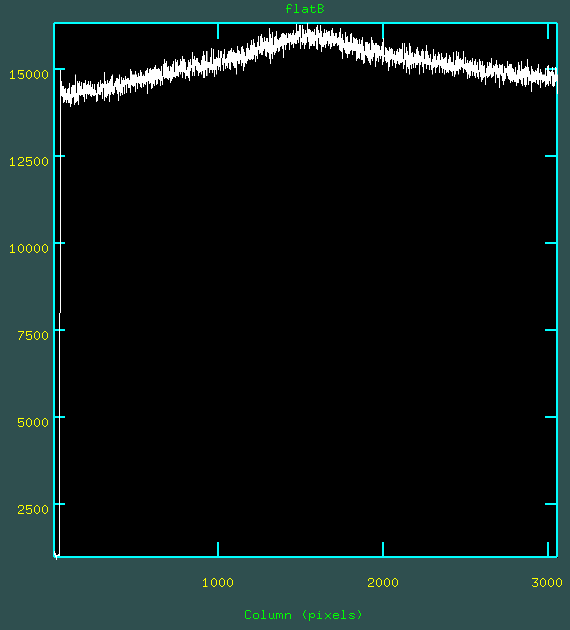
\includegraphics[width=\linewidth,height=0.28\textheight,keepaspectratio]{imagenes/perfil_antes_colbias.png}
\caption{Perfil horizontal del dome flat B antes de aplicar \texttt{colbias}
antes de aplicar \texttt{colbias}. Se observa el salto en las columnas
1:35 correspondiente al overscan de columnas (nivel $\approx 1020$ ADU).}
\label{fig:antes_colbias}
\end{figure}

\begin{figure}[ht]
\centering
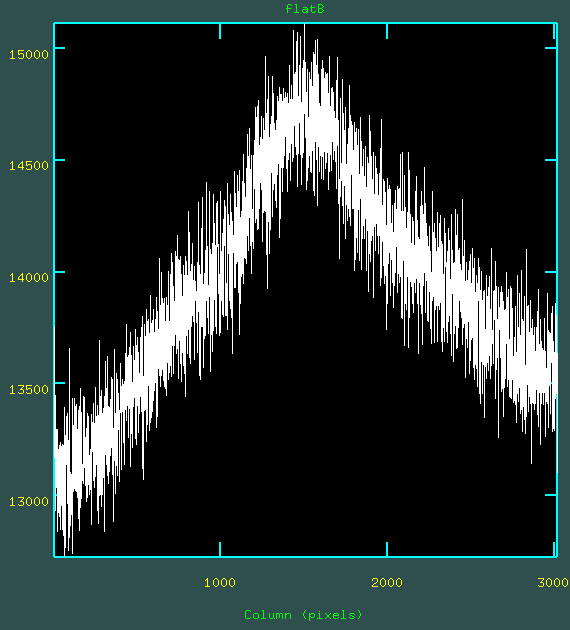
\includegraphics[width=\linewidth,height=0.28\textheight,keepaspectratio]{imagenes/perfil_despues_colbias.png}
\caption{Perfil horizontal de \texttt{TrmFlatB001.fits} después de aplicar
\texttt{colbias}. La franja de overscan de columnas ha sido sustraída y
recortada. La forma de domo observada corresponde al gradiente de
iluminación del dome flat.}
\label{fig:despues_colbias}
\end{figure}

\subsubsection{Corrección de la segunda región (filas) con \texttt{linebias}}

{\raggedright
En la imagen recortada en columnas \texttt{TrmFlatB001.fits}, de 3021
columnas por 3056 filas, se aplicó \texttt{linebias} para corregir el
overscan de filas:
\par}

\begin{lstlisting}
unlearn linebias
linebias TrmFlatB001.fits Trm2FlatB001.fits \
  bias="[1:3021,1:20]" trim="[1:3021,21:3056]" \
  function=chebyshev order=1 interactive=no median=no \
  low_rej=3. high_re=3.
\end{lstlisting}

Las Figuras~\ref{fig:antes_linebias} y~\ref{fig:despues_linebias} comparan
los perfiles verticales antes y después de \texttt{linebias}. El perfil
inicial muestra el salto en las filas 1:20; la imagen final,
\texttt{Trm2FlatB001.fits}, ya no contiene las regiones de overscan.

\begin{figure}[ht]
\centering
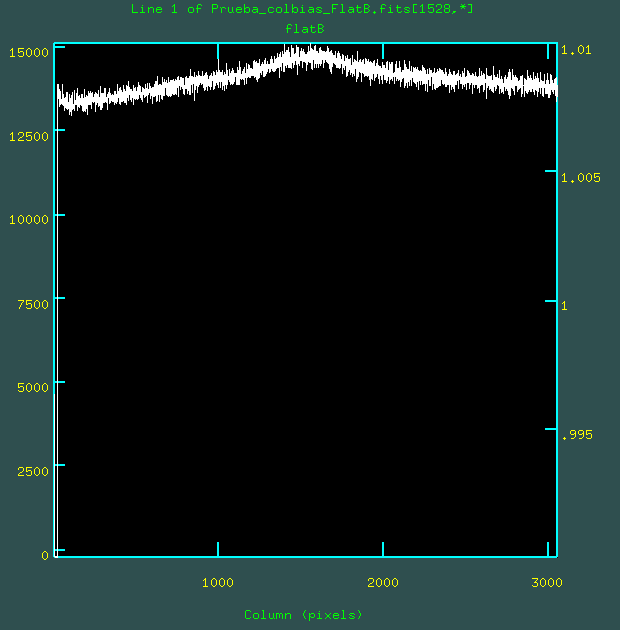
\includegraphics[width=\linewidth,height=0.28\textheight,keepaspectratio]{imagenes/perfil_antes_linebias.png}
\caption{Perfil vertical de \texttt{TrmFlatB001.fits} antes de aplicar
\texttt{linebias}. Se observa el salto en las filas 1:20 correspondiente
al overscan de filas (nivel $\approx 1208$ ADU).}
\label{fig:antes_linebias}
\end{figure}

\begin{figure}[ht]
\centering
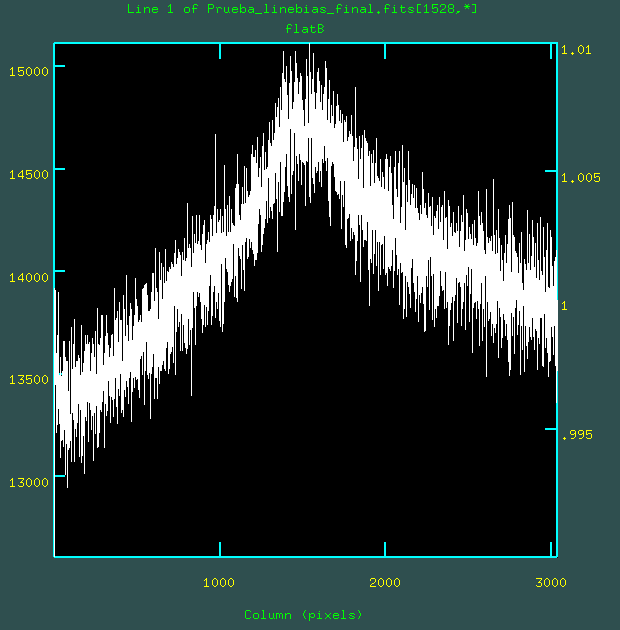
\includegraphics[width=\linewidth,height=0.28\textheight,keepaspectratio]{imagenes/perfil_despues_linebias.png}
\caption{Perfil vertical de \texttt{Trm2FlatB001.fits} después de aplicar
\texttt{linebias}. Ambas regiones de overscan han sido sustraídas y
recortadas. La imagen final tiene dimensiones 3021 $\times$ 3036 píxeles.}
\label{fig:despues_linebias}
\end{figure}

\subsubsection{Aplicación por lotes a todas las imágenes}

Una vez verificados los parámetros con la imagen de prueba, se procesaron
las 65 imágenes (47 bias, 5 darks, 5 flats B, 5 flats V y 2 ciencias)
mediante un script \texttt{overscan\_lote.cl}:

\begin{lstlisting}
# overscan_lote.cl
noao
imred
bias

!ls Bias/Zero.fits Bias/domeflat_Bias_1_secs_*.fits Dark/*.fits \
  domeflat_B/*.fits domeflat_V/*.fits MEL25*.fits > input
!sed 's|.*/||; s|^|Trm|' input > output

colbias @input @output bias="[1:35,21:3056]" trim="[36:3056,1:3056]" \
  function=chebyshev order=1 interactive=no median=no \
  low_rej=3. high_re=3.

!ls Trm*.fits > input2
!sed 's|^|Lb|' input2 > output2

linebias @input2 @output2 bias="[1:3021,1:20]" trim="[1:3021,21:3056]" \
  function=chebyshev order=1 interactive=no median=no \
  low_rej=3. high_re=3.

!ls Lb*.fits
\end{lstlisting}

\subsection{Supercalibraciones (Paso 4)}

\subsubsection{Tareas de combinación y uso de las cabeceras}

{\raggedright
\texttt{imcombine} combina imágenes píxel a píxel y permite promediar,
calcular la mediana o sumar, con rechazo de valores atípicos mediante métodos
como \texttt{avsigclip}, \texttt{minmax} o \texttt{pclip}. Los envoltorios
\texttt{zerocombine}, \texttt{darkcombine} y \texttt{flatcombine}
seleccionan tipos con \texttt{IMAGETYP} (\texttt{ccdtype});
\texttt{zerocombine} no escala bias (\texttt{scale=none}),
\texttt{darkcombine} puede escalar por exposición
(\texttt{scale=exposure}) y \texttt{flatcombine} normaliza por moda o
mediana y agrupa por filtro (\texttt{FILTER}, \texttt{subset}).
Aquí las listas se separaron explícitamente por tipo y filtro. Como
\texttt{darkcombine} y \texttt{flatcombine} dieron errores de archivo de
parámetros en Community IRAF 2.17.1, se usó \texttt{imcombine} con el
escalado indicado manualmente. En ECL, las listas \texttt{@archivo}
deben asignarse a un parámetro (por ejemplo, \texttt{input=@lista}), no
pasarse como argumento posicional.
\par}

\subsubsection{Combinación de bias y darks}

Para el master bias se combinaron los 47 marcos bias corregidos de overscan y
\texttt{LbTrmZero.fits}, con promedio y rechazo sigma iterativo. La bitácora
indica que \texttt{Zero.fits} duplica el marco 001: se usaron 48 archivos,
pero corresponden a 47 marcos únicos. Los cinco darks tienen todos 90 s de
exposición, por lo que no requirieron escalado temporal:

\begin{lstlisting}
noao
imred
ccdred
unlearn zerocombine
!ls LbTrmdomeflat_Bias_1_secs_*.fits LbTrmZero.fits > lista_bias.txt
zerocombine input=@lista_bias.txt output=MasterBias.fits \
  combine=average reject=avsigclip scale=none
imhead MasterBias.fits
imstat MasterBias.fits
display MasterBias.fits 1 fill+ zscale-

!ls LbTrmMEL25_Dark_90_secs_*.fits > lista_dark.txt
imcombine input=@lista_dark.txt output=MasterDark.fits \
  combine=average reject=avsigclip scale=none
imhead MasterDark.fits
imstat MasterDark.fits
display MasterDark.fits 2 fill+ zscale-
\end{lstlisting}

\subsubsection{Combinación y normalización de flats}

Los cinco dome flats de cada filtro se inspeccionaron individualmente en
DS9. No se descartaron marcos: no presentaban estrellas superpuestas ni
saturación, y mostraban gradientes suaves y reproducibles. Sus máximos
individuales eran de aproximadamente $1.6\times10^{4}$ ADU, por debajo
del límite de 65535 del formato ushort. Se combinaron por filtro con
\texttt{scale=mode}; luego cada master se dividió por su media de
\texttt{imstat} (13458 ADU en B y 13177 ADU en V) para obtener media
uno en las imágenes normalizadas.

\begin{lstlisting}
!ls LbTrmdomeflat_Flat_B_90_secs_*.fits > lista_flat_B.txt
imcombine input=@lista_flat_B.txt output=MasterFlat_B.fits \
  combine=average reject=avsigclip scale=mode
!ls LbTrmdomeflat_Flat_V_40_secs_*.fits > lista_flat_V.txt
imcombine input=@lista_flat_V.txt output=MasterFlat_V.fits \
  combine=average reject=avsigclip scale=mode

imarith MasterFlat_B.fits / 13458. MasterFlat_B_norm.fits
imarith MasterFlat_V.fits / 13177. MasterFlat_V_norm.fits
imstat MasterFlat_B_norm.fits
imstat MasterFlat_V_norm.fits
\end{lstlisting}


\subsection{Reducción de imágenes de ciencia (Paso 5)}

Aunque no estaba descrito explicitamente en las instrucciones, las imágenes Flat de los filtros B y V se corrigieron inicialmente por Bias y Dark. Para el filtro V, debido a que las exposiciones fueron de 40 s y los darks disponibles eran de 90 s, se escaló el MasterDark mediante el factor $40/90$. Posteriormente, se combinaron las cinco imágenes corregidas de cada filtro utilizando \texttt{imcombine}, con el método de promedio (\texttt{average}) y rechazo de valores atípicos (\texttt{avsigclip}), obteniendo los respectivos MasterFlat.

Los MasterFlat se normalizaron utilizando su moda, cuyos valores fueron 13742 ADU para B y 13590 ADU para V. Finalmente, las imágenes científicas corregidas por Bias y Dark se dividieron por sus respectivos MasterFlat normalizados. Este procedimiento permitió corregir las variaciones de iluminación y sensibilidad entre los píxeles del detector.\\

Para lo anterior se usaron los siguientes comandos:\\

\noindent\textbf{Comandos IRAF utilizados}

{\footnotesize
\begin{verbatim}
# Escalar MasterDark para V
imarith MasterDark_nuevo.fits * 0.444444
        MasterDark_V_40s.fits

# Combinar Flat B y V
imcombine @lista_flat_B.txt MasterFlat_B_cal.fits
combine=average reject=avsigclip scale=none

imcombine @lista_flat_V.txt MasterFlat_V_cal.fits
combine=average reject=avsigclip scale=none

# Consultar estadísticas
imstat MasterFlat_B_cal.fits
imstat MasterFlat_V_cal.fits

# Normalizar por la moda
imarith MasterFlat_B_cal.fits / 13742
        MasterFlat_B_norm_moda.fits

imarith MasterFlat_V_cal.fits / 13590
        MasterFlat_V_norm_moda.fits

# Aplicar corrección Flat
imarith Light_B_Cal.fits / MasterFlat_B_norm_moda.fits
        Light_B_Final.fits

imarith Light_V_Cal.fits / MasterFlat_V_norm_moda.fits
        Light_V_Final.fits
\end{verbatim}
}

\noindent\textbf{Cálculo de la reducción del ruido de fondo}

La reducción porcentual del ruido se calculó mediante:

\[
R(\%)=
\frac{\sigma_{\mathrm{original}}-\sigma_{\mathrm{calibrada}}}
{\sigma_{\mathrm{original}}}\times 100
\]

donde $\sigma$ corresponde a la desviación estándar de las intensidades
de los píxeles en una región del fondo del cielo.


Esto se obtuvo mediante el comando
\texttt{imstat}, utilizando el parámetro \texttt{STDDEV} sobre regiones
de $101\times101$ píxeles de las imágenes originales y calibradas.
Los valores obtenidos se emplearon para calcular la reducción porcentual
del ruido de fondo.

{\scriptsize
\begin{verbatim}
imstat imagen_original_B.fits
[1398:1498,1210:1310]
imstat Light_B_Final.fits
[1398:1498,1210:1310]

imstat imagen_original_V.fits
[1266:1366,1168:1268]
imstat Light_V_Final.fits
[1266:1366,1168:1268]
\end{verbatim}
}

\section{Resultados}
\subsection{Ganancia y ruido de lectura}
\begin{table}[ht]
\centering
\caption{Resultados del método de la varianza de diferencias por filtro.}
\label{tab:ganancia}
\begin{tabular}{lcc}
\toprule
Cantidad & Filtro B & Filtro V \\
\midrule
$\bar{F}$ (ADU)              & 15464.78 & 15223.71 \\
$\bar{B}$ (ADU)              & 1005.50  & 1006.33  \\
$S=\bar{F}-\bar{B}$ (ADU)    & 14459.28 & 14217.37 \\
$\sigma^2_F$ (ADU$^2$)       & 10049.80 & 9835.71  \\
$\sigma^2_B$ (ADU$^2$)       & 44.10    & 45.18    \\
\midrule
$g$ (e$^-$/ADU)              & 1.445    & 1.452    \\
RN (e$^-$)                   & 9.60     & 9.76     \\
\bottomrule
\end{tabular}
\end{table}

\noindent\textbf{Valor adoptado:} $g = 1.45 \pm 0.01$~e$^-$/ADU y
RN $= 9.7 \pm 0.1$~e$^-$. El acuerdo entre filtros (menor al 2\,\%) es
esperable, pues ambos parámetros son propiedades del detector y su
electrónica, no del filtro; esto valida el método. Como verificación, la
varianza de disparo esperada $S/g \approx 10006$~ADU$^2$ reproduce la
varianza del flat una vez restado el aporte de lectura ($\sigma^2_F -
\sigma^2_B$).

\subsection{Verificación de la corrección del overscan}
\noindent La verificación final confirmó que todas las imágenes
\texttt{LbTrm*.fits} tienen dimensiones [3021,3036] y carecen de las
franjas de overscan visibles en las imágenes originales.

\subsection{Supercalibraciones (Paso 4)}

\subsubsection{Master bias y master dark}

El master bias tiene media de 0.26 ADU, consistente con el nivel de lectura
removido durante la corrección de overscan, y desviación estándar de 2.36 ADU.
El análisis de los avances estima que el componente aleatorio de esta
dispersión sería $6.64/\sqrt{48}\approx0.96$ ADU, además de un patrón fijo de
columnas de aproximadamente 2.15 ADU, visible entre $-7.8$ y 15.5 ADU. La
estimación de 0.96 ADU supone 48 marcos independientes; dado que uno de los
archivos duplica el marco 001, debe tomarse como valor nominal. El máximo de
1509 ADU corresponde a píxeles calientes persistentes que el rechazo
\texttt{avsigclip} no elimina al no ser atípicos dentro de la combinación.

El master dark presenta una media de 0.36 ADU en 90 s, equivalente a
$\sim0.004$ ADU s$^{-1}$ o $\sim0.006$ e$^{-}$ s$^{-1}$ usando
$g=1.45$ e$^{-}$/ADU. A $-25\,^{\circ}$C, la corriente oscura es despreciable
frente al ruido de lectura, aunque se conserva la corrección por rigor
metodológico. Su desviación estándar de 49.6 ADU y el máximo de 64526 ADU
están dominados por píxeles calientes persistentes; el componente aleatorio
esperado para cinco marcos es $6.64/\sqrt{5}\approx2.97$ ADU.

\subsubsection{Master flats por filtro}

Las modas individuales y los factores de escala aplicados con
\texttt{scale=mode} se resumen en la Tabla~\ref{tab:modas_master}. Las modas
se encuentran entre 13471 y 13786 ADU y los factores entre 0.995 y 1.006.
Las modas de los marcos coinciden con la media del master dentro de aproximadamente 2\%.
Aunque la consigna propone normalizar respecto a la moda, en este
procesamiento se dividieron los masters por sus medias \texttt{imstat}
(13458 ADU en B y 13177 ADU en V), de modo que la media de cada flat
normalizado sea exactamente 1.000.

\begin{table}[ht]
\centering
\caption{Modas y factores de escala aplicados por \texttt{imcombine}
(\texttt{scale=mode}) a cada dome flat.}
\label{tab:modas_master}
\scriptsize
\setlength{\tabcolsep}{1.5pt}
\begin{tabular}{lrr|lrr}
\toprule
Marco (B) & Moda (ADU) & Escala & Marco (V) & Moda (ADU) & Escala \\
\midrule
B001 & 13716 & 1.000 & V001 & 13547 & 1.000 \\
B002 & 13741 & 0.998 & V002 & 13568 & 0.998 \\
B003 & 13786 & 0.995 & V003 & 13593 & 0.997 \\
B004 & 13775 & 0.996 & V004 & 13585 & 0.997 \\
B005 & 13767 & 0.996 & V005 & 13471 & 1.006 \\
\bottomrule
\end{tabular}
\end{table}

Los flats normalizados tienen desviaciones estándar de 0.076 (B) y 0.079
(V), equivalentes a variaciones relativas de 7.6--7.9\% por el gradiente de
iluminación y el viñeteo. Sus mínimos son 0.013 (B) y 0.007 (V), mientras que
los máximos 4.77 y 4.88 corresponden a defectos residuales presentes en todos
los marcos.

\subsubsection{Estadísticas e inspección visual}

La Tabla~\ref{tab:estadisticas_supercalibraciones} presenta las estadísticas
de \texttt{imstat} para los masters y los flats normalizados. Todas las
imágenes tienen 9\,171\,756 píxeles y dimensiones $3021\times3036$.

\begin{table}[ht]
\centering
\caption{Estadísticas de \texttt{imstat} de las supercalibraciones y los
flats normalizados.}
\label{tab:estadisticas_supercalibraciones}
\scriptsize
\setlength{\tabcolsep}{1.5pt}
\begin{tabular}{>{\raggedright\arraybackslash}p{1.6cm}rrrrr}
\toprule
Imagen & $N$ & Media & Desv. & Mín & Máx \\
\midrule
MasterBias          & 48 & 0.2641 & 2.358   & $-23.83$ & 1509    \\
MasterDark          & 5  & 0.3645 & 49.57   & $-33.37$ & 64526   \\
MasterFlat B       & 5  & 13458  & 1019    & 171.5    & 64137   \\
MasterFlat V       & 5  & 13177  & 1040    & 95.41    & 64293   \\
MasterFlat B norm & 5  & 1.000  & 0.0757  & 0.01274  & 4.766   \\
MasterFlat V norm & 5  & 1.000  & 0.07894 & 0.007241 & 4.879   \\
\bottomrule
\end{tabular}
\end{table}

En la inspección conjunta (Figura~\ref{fig:supercalibraciones}), el master bias muestra un patrón fijo de columnas; el dark, píxeles calientes aislados sobre el fondo; y los flats conservan el gradiente de iluminación y el viñeteo en las esquinas.

\begin{figure}[t]
\centering
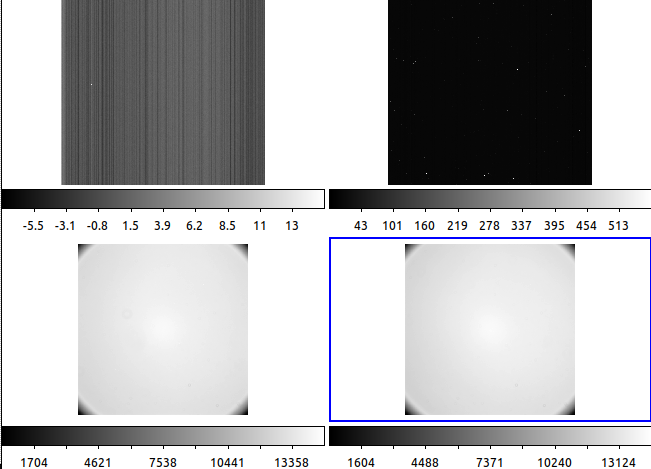
\includegraphics[width=\linewidth,height=0.22\textheight,keepaspectratio]{imagenes/supercalibraciones_ds9.png}
\caption{Inspección en DS9 (\texttt{fill+ zscale-}) de las cuatro supercalibraciones. Arriba izquierda: MasterBias ($z=-7.8$ a 15.5 ADU); arriba derecha: MasterDark ($z=-15.7$ a 571.5 ADU); abajo izquierda: MasterFlat\_B ($z=252.2$ a 14810 ADU); abajo derecha: MasterFlat\_V ($z=169.4$ a 14559 ADU).}
\label{fig:supercalibraciones}
\end{figure}

\noindent\textbf{Lectura conjunta.} El master bias confirma que la
corrección de overscan centró el nivel de lectura alrededor de cero; el
master dark muestra que a $-25\,^{\circ}$C la corriente oscura es pequeña
frente al ruido de lectura; y los flats normalizados conservan la respuesta
relativa del sistema, lista para corregir las imágenes científicas en el paso
siguiente.

\subsection{Reducción de imágenes de ciencia}

En la figura \ref{fig:antes_despues_V} se muestra, visualizada en DS9, la imagen de MEL25 en el filtro V antes y después de la reducción (resta de bias y dark, y división por el flat normalizado, realizadas con \texttt{imarith}). A la izquierda se ve la imagen cruda y a la derecha la imagen reducida.\\

% Preámbulo: \usepackage{graphicx}
Análogamente, en la figura \ref{fig:antes_despues_B} se muestra   la imagen de MEL25 en el filtro B antes y después de la reducción (resta de bias y dark, y división por el flat normalizado, realizadas con \texttt{imarith}). A la izquierda se ve la imagen cruda y a la derecha la imagen reducida.\\
% Preámbulo:
% \usepackage{graphicx}
% \usep
\medskip


\subsubsection{Cálculo de reducción de ruido de fondo}
Para el filtro B se obtuvieron los siguientes resultados:

\begin{table}[h!]
\centering
\caption{Estadísticas del fondo para el filtro B.}
\begin{tabular}{lcc}
\hline
\textbf{Parámetro} & \textbf{Original} & \textbf{Calibrada} \\
\hline
Número de píxeles & 10201 & 10201 \\
Media (ADU) & 1015 & 1.025 \\
Desviación estándar (ADU) & 16.63 & 7.333 \\
\hline
\end{tabular}
\end{table}

La reducción porcentual del ruido para el filtro B fue:

\[
R_B =
\frac{16.63-7.333}{16.63}\times 100
= \boxed{55.91\%}
\]

\medskip
\noindent\textbf{Filtro V}

Para el filtro V se obtuvieron los siguientes resultados:

\begin{table}[h!]
\centering
\caption{Estadísticas del fondo para el filtro V.}
\begin{tabular}{lcc}
\hline
\textbf{Parámetro} & \textbf{Original} & \textbf{Calibrada} \\
\hline
Número de píxeles & 10201 & 10201 \\
Media (ADU) & 1021 & 2.099 \\
Desviación estándar (ADU) & 44.38 & 7.693 \\
\hline
\end{tabular}
\end{table}

La reducción porcentual del ruido para el filtro V fue:

\[
R_V =
\frac{44.38-7.693}{44.38}\times 100
= \boxed{82.67\%}
\]

\medskip
\noindent\textbf{Comparación de resultados}

\begin{table}[h!]
\centering
\caption{Reducción del ruido de fondo en ambos filtros.}
\begin{tabular}{lccc}
\hline
\textbf{Filtro} &
$\boldsymbol{\sigma_{\mathrm{antes}}}$ &
$\boldsymbol{\sigma_{\mathrm{después}}}$ &
\textbf{Reducción (\%)} \\
\hline
B & 16.63 & 7.333 & 55.91 \\
V & 44.38 & 7.693 & 82.67 \\
\hline
\end{tabular}
\end{table}

Los resultados muestran una disminución de la desviación estándar
del fondo del cielo en ambos filtros después de la calibración.
El filtro B presentó una reducción del ruido del 55.91\%,
mientras que el filtro V alcanzó una reducción del 82.67\%.
Esto evidencia una disminución de la dispersión de los valores
de intensidad en las regiones de cielo analizadas.


\onecolumn
\begin{figure}[htbp]
\centering
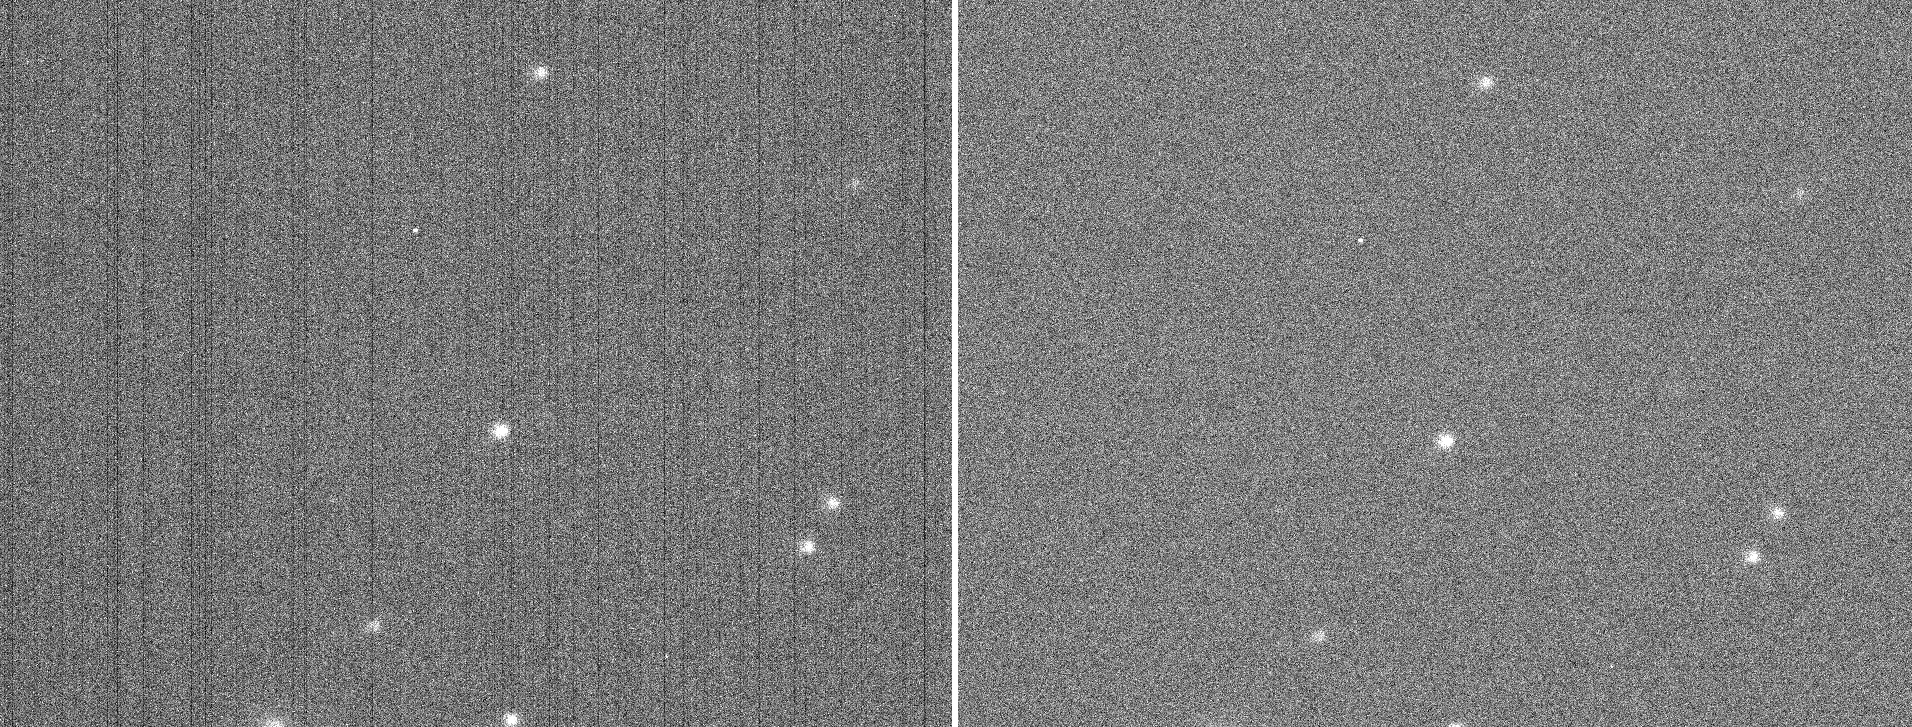
\includegraphics[width=\textwidth]{imagenes/mel25_V_antes_despues.png}
\caption{Imagen de MEL25 en el filtro V antes (izquierda) y después (derecha) de la reducción con bias, dark y flat.}
\label{fig:antes_despues_V}
\end{figure}




\onecolumn
\begin{figure}[htbp]
\centering
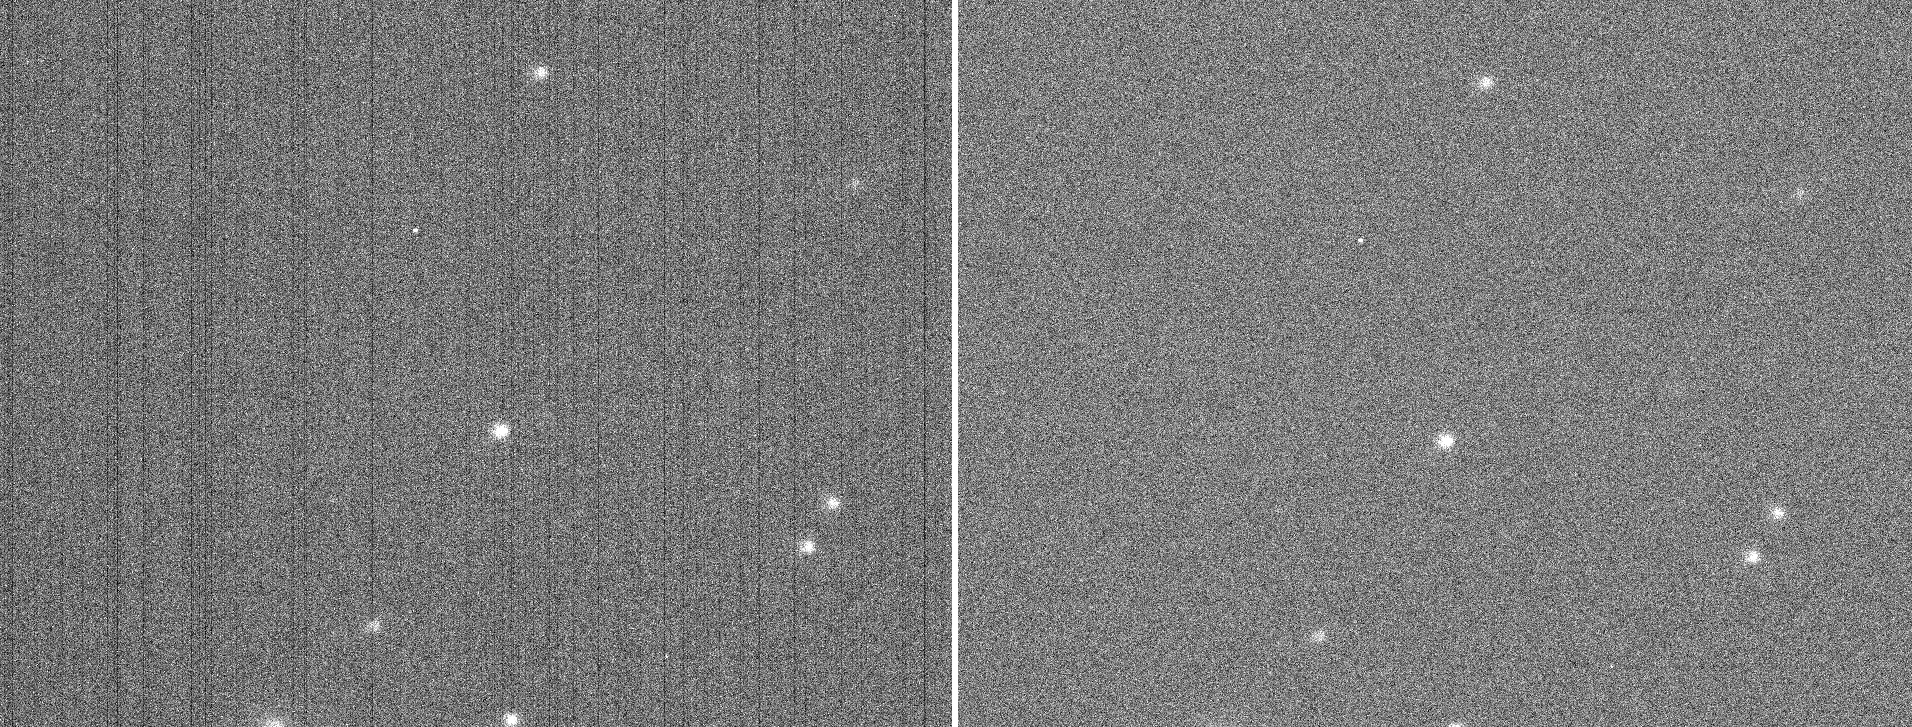
\includegraphics[width=\textwidth]{imagenes/mel25_B_antes_despues.png}
\caption{Imagen de MEL25 en el filtro B antes (izquierda) y después (derecha) de la reducción con bias, dark y flat.}
\label{fig:antes_despues_B}
\end{figure}

 

\section{Conclusiones}
% Pendiente de desarrollar.

\section*{Referencias}
% Agregar aquí las referencias utilizadas.

\end{document}